\newpage
\section{Test of the Reverb Effect}
In this part, tests for the reverb effect that show whether it fulfils the requirements are presented. 


\subsection{Test of \autoref{req:reverb1}}
According to \autoref{req:reverb1}, a test was made to ensure that the \gls{reverb} have at least 1000 echoes. The test is made by sending a single known sine impulse into the \gls{reverb} effect. The test setup is shown in \autoref{chap:effect_test_response}. Ideally every echo should have been counted, but the scope have a limitation of 16k samples on each measurement screen, which complicates the measurement. Instead measurements at different frequencies will be compared to the equivalent MATLAB coded \gls{reverb} simulations. The MATLAB simulation and the measurement will be situated side by side. This is done with five different frequencies with the frequencies \SI{20}{\hertz}, \SI{50}{\hertz}, \SI{200}{\hertz}, \SI{1}{\kilo\hertz}, and \SI{5}{\kilo\hertz} in \autoref{fig:tests:reverb:20Hz}, \autoref{fig:tests:reverb:50Hz}, \autoref{fig:tests:reverb:200Hz}, \autoref{fig:tests:reverb:1kHz}, and \autoref{fig:tests:reverb:5kHz}. 

\subsubsection*{Impulse response of \SI{20}{\hertz}}


\begin{figure}[htbp!]
    \centering
        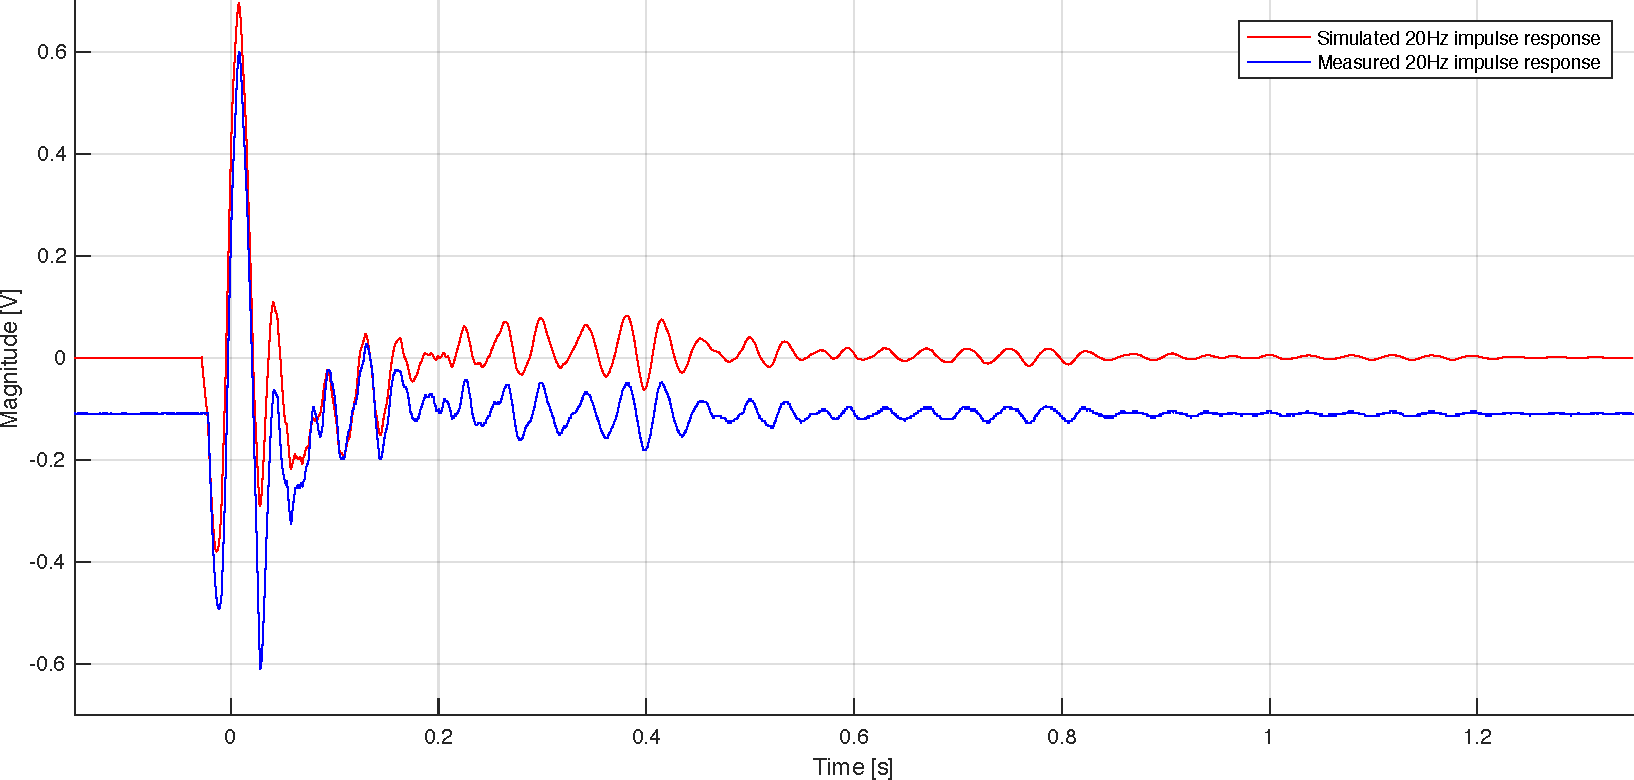
\includegraphics[width=\textwidth]{20Hz_impulse_response.pdf}
        \caption{Plot of the measured and simulated \gls{reverb} impulse response at \SI{20}{\hertz}.}
        \label{fig:tests:reverb:20Hz}
  \end{figure}
  
  \newpage
  
\subsubsection*{Impulse response of \SI{50}{\hertz}}

\begin{figure}[htbp!]
    \centering
        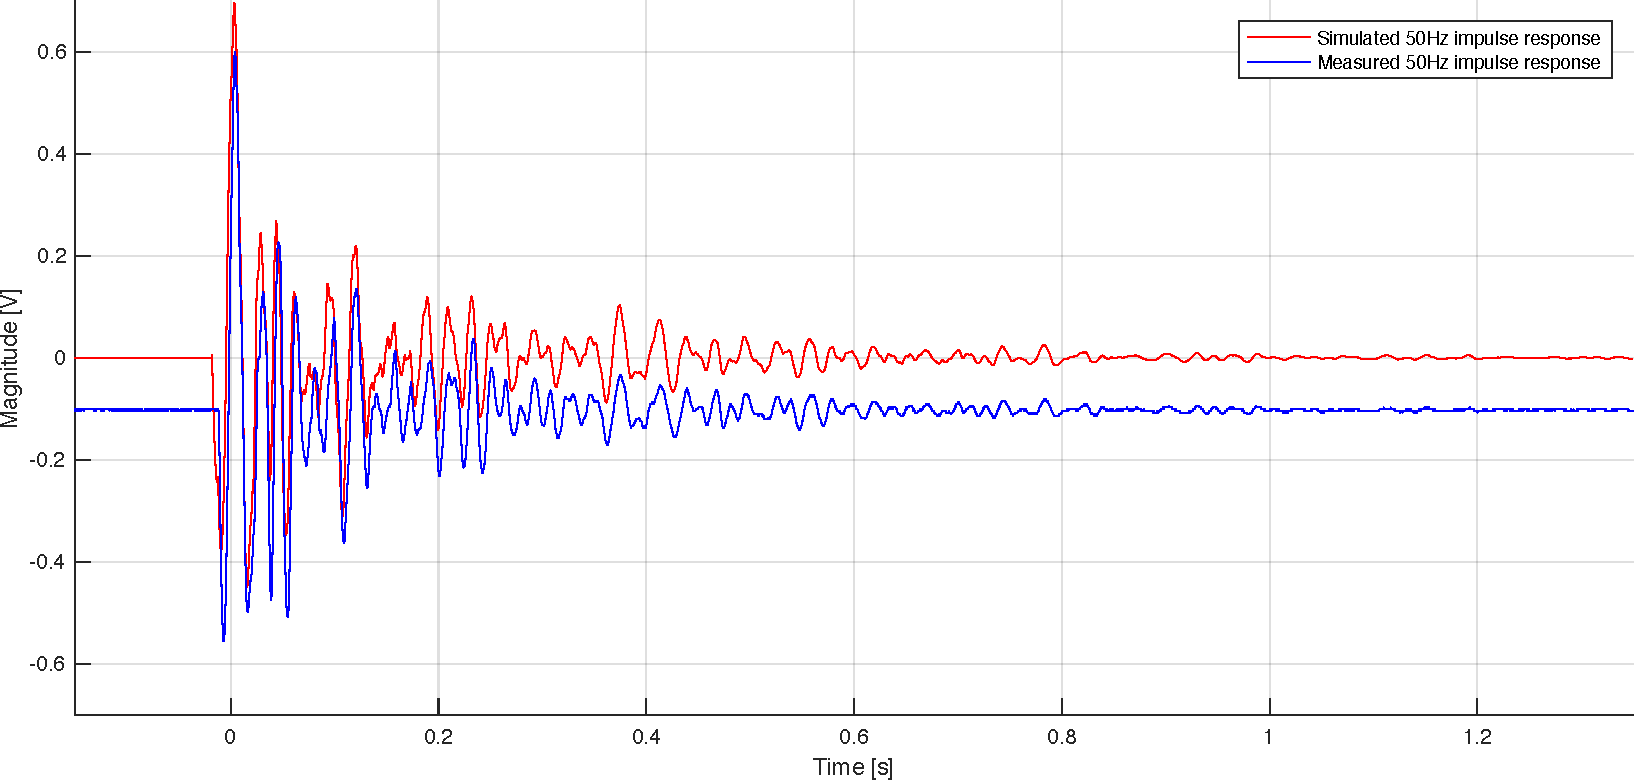
\includegraphics[width=\textwidth]{50Hz_impulse_response.pdf}
        \caption{Plot of the measured and simulated \gls{reverb} impulse response at \SI{50}{\hertz}.}
        \label{fig:tests:reverb:50Hz}
  \end{figure}

\subsubsection*{Impulse response of \SI{200}{\hertz}}

\begin{figure}[htbp!]
    \centering
        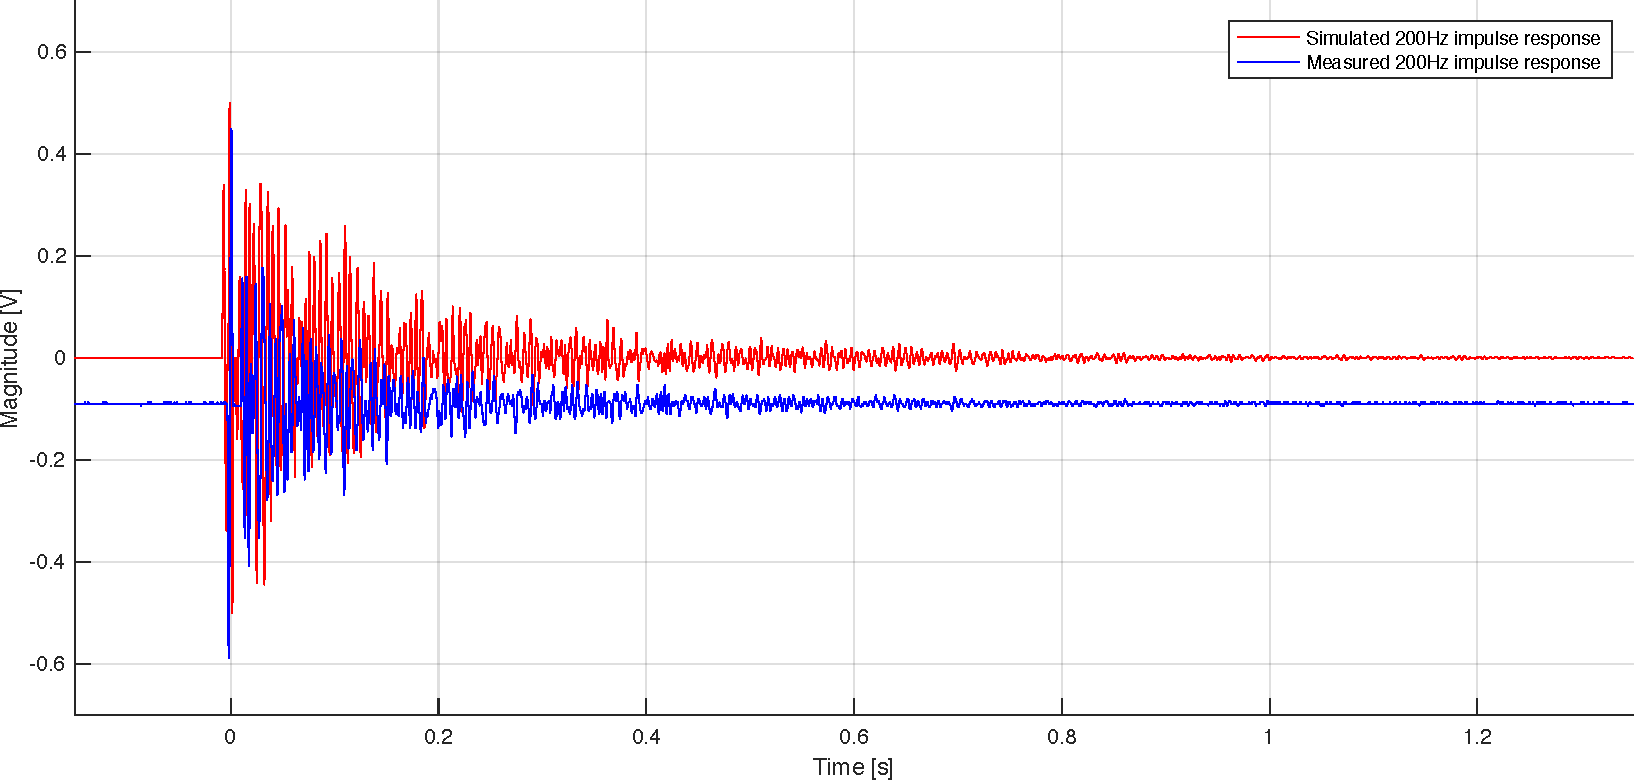
\includegraphics[width=\textwidth]{200Hz_impulse_response.pdf}
        \caption{Plot of the measured and simulated \gls{reverb} impulse response at \SI{200}{\hertz}.}
        \label{fig:tests:reverb:200Hz}
  \end{figure}

  \newpage
\subsubsection*{Impulse response of \SI{1}{\kilo\hertz}}

\begin{figure}[htbp!]
    \centering
        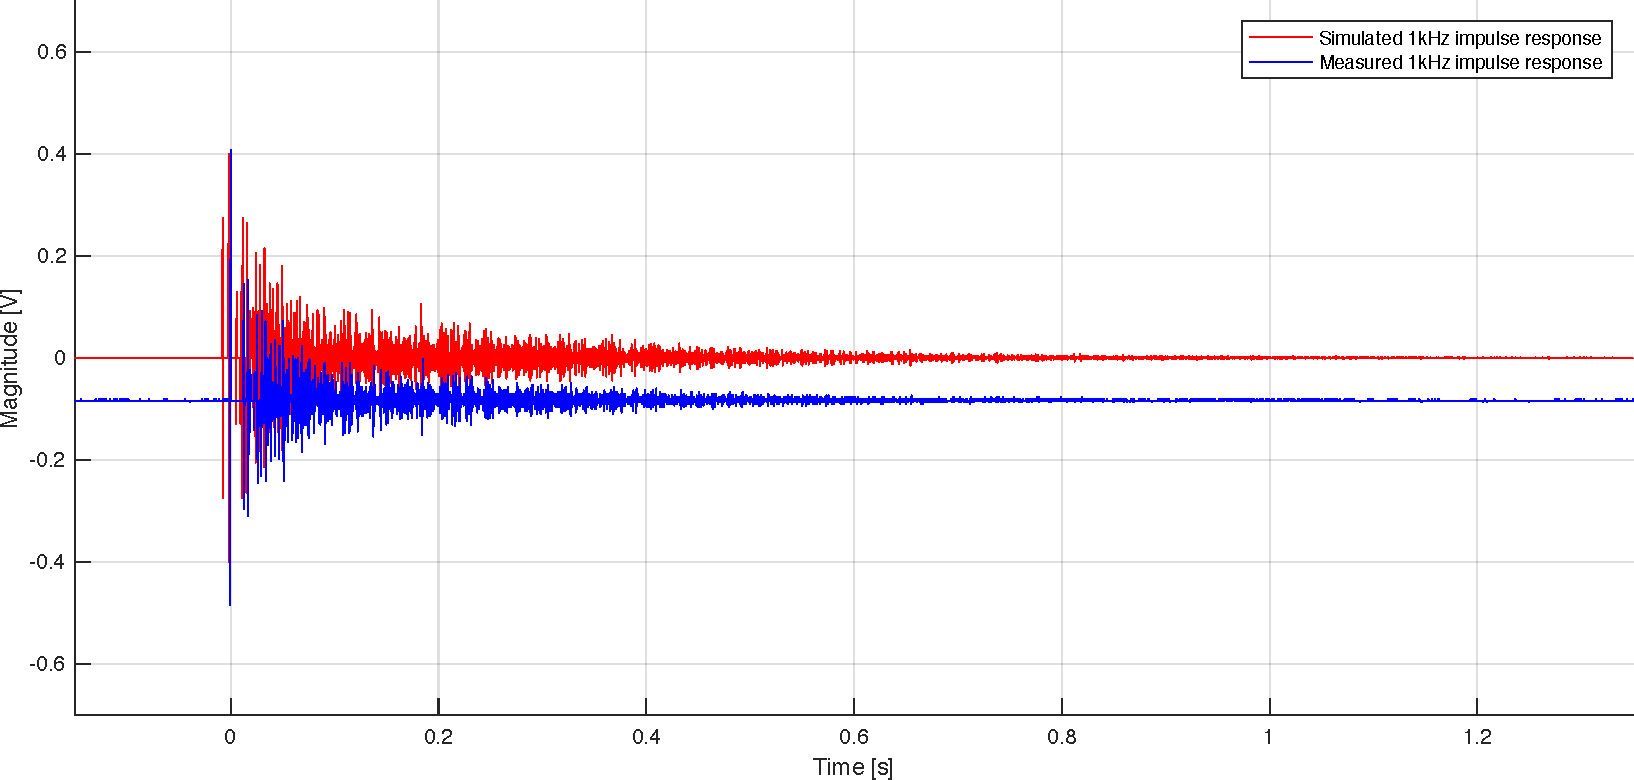
\includegraphics[width=\textwidth]{1kHz_impulse_response.pdf}
        \caption{Plot of the measured and simulated \gls{reverb} impulse response at \SI{1}{\kilo\hertz}.}
        \label{fig:tests:reverb:1kHz}
  \end{figure}
  
  
 \subsubsection*{Impulse response of \SI{5}{\kilo\hertz}}

\begin{figure}[htbp!]
    \centering
        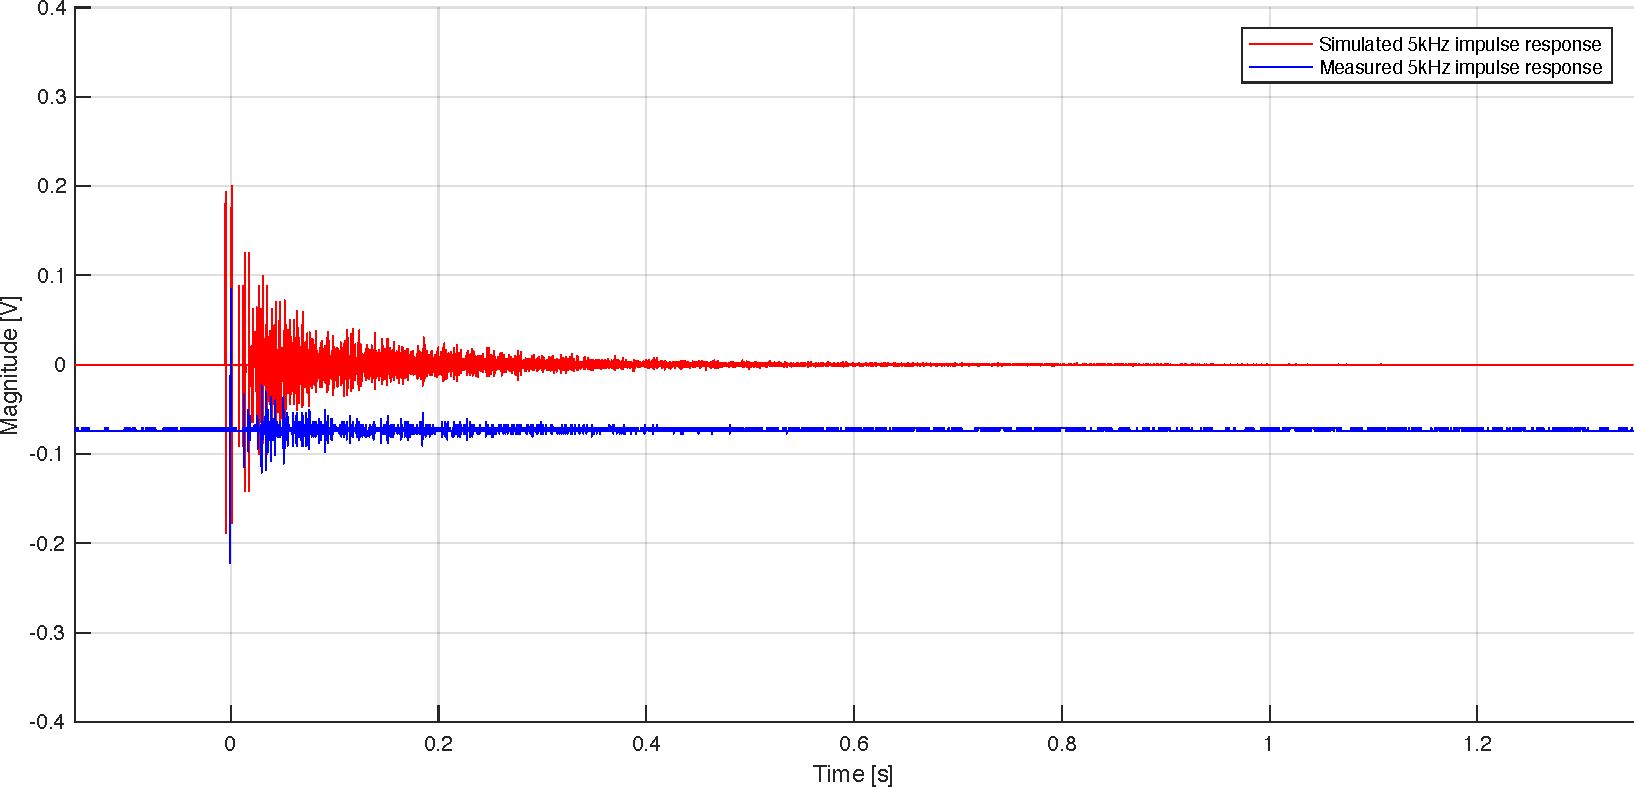
\includegraphics[width=\textwidth]{5kHz_impulse_response.pdf}
        \caption{Plot of the measured and simulated \gls{reverb} impulse response at \SI{5}{\kilo\hertz}.}
        \label{fig:tests:reverb:5kHz}
  \end{figure}
  
According to \autoref{sec:reverb_develop} the simulated data has more 1000 echo, and since the measured data are closely equal to the simulated data, \autoref{req:reverb1} is approved
  
  
\subsection{Test of \autoref{req:reverb2}}
According to \autoref{fig:reverb_block_design} there is a gain called wet and dry, which is able to adjust the factor between the \gls{reverb} effect and the direct sound as following \autoref{eq:test:wetdry}

\begin{subequations}\label{eq:test:wetdry}
\begin{equation}
Dry = \text{user settings}
    \end{equation}
\begin{equation}
Wet = 1-\frac{\text{user settings}}{1} 
    \end{equation}
 \end{subequations}
    \startexplain
     \explain{$\text{user settings}$ is a user defined number between 0 and 1}{\si{1}}
    \stopexplain


Since the user interface not is implemented, \autoref{req:reverb2} is conditionally approved


\subsection{Test of \autoref{req:reverb3}}
According to \autoref{eq:reverb_eq_f} and the following formulas in \autoref{sec:reverb_develop} the gain of every \gls{lpcf} can be changed, which will decrease or increase the number of echoes from the six \gls{lpcf}. Since the user interface has not been implemented, the user is only able to change the number of echoes by changing it directly in the code. Thus \autoref{req:reverb3} is conditionally approved

\subsection{Test Review of the Reverb Effect}
In this subsection, a short review will be shown of the \gls{reverb} effect test.

\begin{table}[H]
\centering
\caption{Recap of the requirements fulfilments for the \gls{reverb} }
\label{test_of_reverb_table}
\begin{tabular}{|l|l|}
\hline
\rowcolor[HTML]{9B9B9B} 
\textbf{Requirement} & \textbf{Fulfilment State} \\ \hline
\textbf{\ref{req:reverb1}}    & \cmark                     \\ \hline
\textbf{\ref{req:reverb2}}    & \cmark*                     \\ \hline
\textbf{\ref{req:reverb3}}    & \cmark*                     \\ \hline
\end{tabular}
\end{table}
